%%%%%%%%%%%%%%%%%%%%%%%%%%%%%%%%%%%%%%%%%
% Arsclassica Article
% LaTeX Template
% Version 1.1 (10/6/14)
%
% This template has been downloaded from:
% http://www.LaTeXTemplates.com
%
% Original author:
% Lorenzo Pantieri (http://www.lorenzopantieri.net) with extensive modifications by:
% Vel (vel@latextemplates.com)
%
% License:
% CC BY-NC-SA 3.0 (http://creativecommons.org/licenses/by-nc-sa/3.0/)
%
%%%%%%%%%%%%%%%%%%%%%%%%%%%%%%%%%%%%%%%%%

%----------------------------------------------------------------------------------------
%	PACKAGES AND OTHER DOCUMENT CONFIGURATIONS
%----------------------------------------------------------------------------------------

\documentclass[
10pt, % Main document font size
a4paper, % Paper type, use 'letterpaper' for US Letter paper
oneside, % One page layout (no page indentation)
%twoside, % Two page layout (page indentation for binding and different headers)
headinclude,footinclude, % Extra spacing for the header and footer
BCOR5mm, % Binding correction
]{scrartcl}

%%%%%%%%%%%%%%%%%%%%%%%%%%%%%%%%%%%%%%%%%
% Arsclassica Article
% Structure Specification File
%
% This file has been downloaded from:
% http://www.LaTeXTemplates.com
%
% Original author:
% Lorenzo Pantieri (http://www.lorenzopantieri.net) with extensive modifications by:
% Vel (vel@latextemplates.com)
%
% License:
% CC BY-NC-SA 3.0 (http://creativecommons.org/licenses/by-nc-sa/3.0/)
%
%%%%%%%%%%%%%%%%%%%%%%%%%%%%%%%%%%%%%%%%%

%----------------------------------------------------------------------------------------
%	REQUIRED PACKAGES
%----------------------------------------------------------------------------------------

\usepackage[
nochapters, % Turn off chapters since this is an article        
beramono, % Use the Bera Mono font for monospaced text (\texttt)
eulermath,% Use the Euler font for mathematics
pdfspacing, % Makes use of pdftex’ letter spacing capabilities via the microtype package
dottedtoc % Dotted lines leading to the page numbers in the table of contents
]{classicthesis} % The layout is based on the Classic Thesis style

\usepackage{arsclassica} % Modifies the Classic Thesis package

\usepackage[T1]{fontenc} % Use 8-bit encoding that has 256 glyphs

\usepackage[utf8]{inputenc} % Required for including letters with accents

\usepackage{graphicx} % Required for including images
\graphicspath{{report_figures/}} % Set the default folder for images

\usepackage{enumitem} % Required for manipulating the whitespace between and within lists

\usepackage{lipsum} % Used for inserting dummy 'Lorem ipsum' text into the template

\usepackage{subfig} % Required for creating figures with multiple parts (subfigures)

\usepackage{amsmath,amssymb,amsthm} % For including math equations, theorems, symbols, etc

\usepackage{varioref} % More descriptive referencing

\usepackage[spanish]{babel} % Define spanish document
%----------------------------------------------------------------------------------------
%	THEOREM STYLES
%---------------------------------------------------------------------------------------

\theoremstyle{definition} % Define theorem styles here based on the definition style (used for definitions and examples)
\newtheorem{definition}{Definition}

\theoremstyle{plain} % Define theorem styles here based on the plain style (used for theorems, lemmas, propositions)
\newtheorem{theorem}{Theorem}

\theoremstyle{remark} % Define theorem styles here based on the remark style (used for remarks and notes)

%----------------------------------------------------------------------------------------
%	HYPERLINKS
%---------------------------------------------------------------------------------------

\hypersetup{
%draft, % Uncomment to remove all links (useful for printing in black and white)
colorlinks=true, breaklinks=true, bookmarks=true,bookmarksnumbered,
urlcolor=webbrown, linkcolor=RoyalBlue, citecolor=webgreen, % Link colors
pdftitle={}, % PDF title
pdfauthor={\textcopyright}, % PDF Author
pdfsubject={}, % PDF Subject
pdfkeywords={}, % PDF Keywords
pdfcreator={pdfLaTeX}, % PDF Creator
pdfproducer={LaTeX with hyperref and ClassicThesis} % PDF producer
}
 % Include the structure.tex file which specified the document structure and layout

\hyphenation{Fortran hy-phen-ation} % Specify custom hyphenation points in words with dashes where you would like hyphenation to occur, or alternatively, don't put any dashes in a word to stop hyphenation altogether

%----------------------------------------------------------------------------------------
%	TITLE AND AUTHOR(S)
%----------------------------------------------------------------------------------------

\title{\normalfont\spacedallcaps{Lenguajes para el desarrollo de aplicaciones móviles}} % The article title

\author{\spacedlowsmallcaps{Diego Trabazo Sardón* 
\& Raul Santoveña Gómez\textsuperscript{1}}} % The article author(s) - author
% affiliations need to be specified in the AUTHOR AFFILIATIONS block

\date{\today} % An optional date to appear under the author(s)

%----------------------------------------------------------------------------------------

\begin{document}

%----------------------------------------------------------------------------------------
%	HEADERS
%----------------------------------------------------------------------------------------

\renewcommand{\sectionmark}[1]{\markright{\spacedlowsmallcaps{#1}}} % The header for all pages (oneside) or for even pages (twoside)
%\renewcommand{\subsectionmark}[1]{\markright{\thesubsection~#1}} % Uncomment when using the twoside option - this modifies the header on odd pages
\lehead{\mbox{\llap{\small\thepage\kern1em\color{halfgray} \vline}\color{halfgray}\hspace{0.5em}\rightmark\hfil}} % The header style

\pagestyle{scrheadings} % Enable the headers specified in this block

%----------------------------------------------------------------------------------------
%	TABLE OF CONTENTS & LISTS OF FIGURES AND TABLES
%----------------------------------------------------------------------------------------

\maketitle % Print the title/author/date block

\setcounter{tocdepth}{2} % Set the depth of the table of contents to show sections and subsections only

\tableofcontents % Print the table of contents

%\listoffigures % Print the list of figures

%\listoftables % Print the list of tables

%----------------------------------------------------------------------------------------
%	ABSTRACT
%----------------------------------------------------------------------------------------
\begin{abstract}
Desde el comienzo de los tiempos de la informática la búsqueda de sistemas fisicamente más pequeños ha sido incesante. Hoy en día disponemos de dispositivos que caben en un bolsillo y gracias a la energía suministrada por baterías ofrecen a sus usuarios horas de autonomía y ofrecen multitud de servicios. Existe por supuesto un mercado de software muy activo que explota sus características. Con tantas opciones y fabricantes como hay en la actualidad para los clientes, no menos grande es el abanico para los desarrolladores. Una ámplia variedad de lenguajes y sistema operativos pueden ser tenidos en cuenta. Se tratan en este documento la plataforma Android utilizando Java y Código Nativo. Además también se explica el uso de los lenguajes de la Web, HTML, CSS y JavaScript a la hora de crear una buena experiencia de usuario.
\end{abstract}


%----------------------------------------------------------------------------------------
%	AUTHOR AFFILIATIONS
%----------------------------------------------------------------------------------------

{\let\thefootnote\relax\footnotetext{* \textit{diego.trabazo@udc.es, Facultad de Informática, UDC}}}

{\let\thefootnote\relax\footnotetext{\textsuperscript{1} \textit{Department of Chemistry, University of Examples, London, United Kingdom}}}

%----------------------------------------------------------------------------------------

\newpage % Start the article content on the second page, remove this if you have a longer abstract that goes onto the second page

%----------------------------------------------------------------------------------------
%	INTRODUCTION
%----------------------------------------------------------------------------------------
\section{Introducción}
El sector de los dispositivos móviles ha crecido de manera muy relevante desde el 2007. No es que antes de esa fecha no hubiese computadoras de pequeño tamaño que incorporasen una batería como fuente de energía principal, una pantalla que sirviese de forma de entrada de información, y no sólo para mostrarla como en un ordenador; o interfaces de usuario distintas al teclado y ratón. Pero en el 2007 Apple dió a conocer el primer smartphone de pantalla táctil \cite{rob_price_how_2015} y varias de sus características cambiaron el mercado. Primero la posibilidad de ser utilizado para visualizar imágenes, vídeos, juegos u otro contenido multimedia. La creación de una tienda de aplicaciones que podían ser escritas por terceros desarrolladores, no sólo por Apple. Y por último estos teléfonos se acompañaban de una tarifa de datos, lo cual hizo que Internet estuviese disponible en todo momento. En el 2010, nuevamente Apple, presentó el iPad \cite{john_d._sutter_apple_2010}, que amplió la pantalla hasta convertirse en un dispositivo muy apropiado para el consumo multimedia.

Hoy en día hay muchas alternativas a la hora de adquirir un teléfono o táblet, pero además el modelo se ha extendido a nuevos productos como los relojes o \textit{smartwatches} o los coches con sistemas de \textit{infotainment}. El software utilizado en estos nuevos dispositivos es una adaptación de los sistemas Android o iOS existentes para estos nuevos formatos. Entre sus características comunes están que el método de entrada princial son o bien la voz o bien los gestos sobre la pantalla. Además son dependientes de un teléfono con el que suelen tener que estar emparejados.

\begin{figure}[h]
\centering 
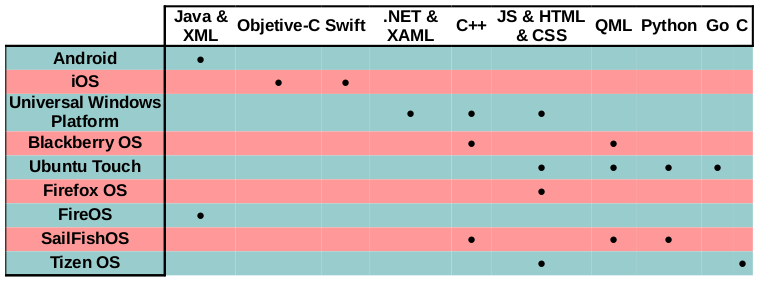
\includegraphics[width=1.1\columnwidth]{report_table_os_lang} 
\caption[Lenguajes recomendados por cada plataforma]{Lenguajes de programación recomendados por cada plataforma.} 
\label{fig:os_lang} 
\end{figure}

Para hacerse una idea de qué lenguajes se pueden utilizar en cuál plataforma basta mirar la figura \vref{fig:os_lang} que refleja las opciones recomendadas por el desarrollador de cada plataforma. No pretende ser exaustiva, pero si dar una idea de que es lo recomendado. Mencionar de forma especial, ya que llama la atención, que en Tizen las aplicaciones nativas se escriban en lenguaje C. No se esperaba a priori que se hiciese uso de lenguajes no Orientados a Objetos para el desarrollo de aplicaciones. Téngase en cuenta que las interfaces de usuario siguen el paradigma de la Orientación a Eventos. El desarrollador define métodos Callback que son llamados por el sistema o por otros métodos de la aplicación de forma automática ante una circunstancia determinada.

%----------------------------------------------------------------------------------------
%	HTML
%----------------------------------------------------------------------------------------
\section{Html: ¿multiplataforma?}
Una opción a considerar a la hora de desarrollar aplicaciones Web modernas es el conjunto de lenguajes habituales de la Web: Html 5, CSS y JavaScript. Es posible contruir y distribuir aplicaciones usando estos tres lenguajes pero hay una serie de aspectos, que se verán a continuación y que conviene tener en cuenta. Los objetivos que se suelen persegir con este enfoque son tanto económicos como tecnológicos: 

\begin{itemize}
\item Disponibilidad multiplataforma: Una misma aplicación debería poder funcionar el todas las plataformas en las que la empresa quiera estar presente.
\item Aprovechamiento de los conocimientos de los desarrolladores existentes en la organización para abarcar un ámbito nuevo y diferente a la Web tradicional.
\item Aprovechar el esfuerzo ya realizado cuando se creó la web de la organización.
\end{itemize}

Los principio de separación de aspecto y comportamiento siguen siendo perfectamente válidos en la Web de hoy en día con HTML 5 y CSS 3. El primero es un lenguaje de marcado cuya principal misión es crear la estructura donde los elementosde la web tienen que ser colocados. Se dota al contenido de contexto, quedando claro que es cada cosa. Con CSS se trabaja todo lo relativo al aspecto final: colores, fuentes o tipografías, maquetación. Un concepto central a CSS es el \textit{Box Model} que agrupa los elementos de la página dentro de cajas que se pueden colocar de distintas maneras o se comportan de distintas maneras dependiendo del dispositivo de visualización.

\subsection{1ª aproximación: WebView / UIWebView / WebBrowser}
En primer lugar y de manera básica, todas las plataformas disponen de algún \textit{browser engine} del cual el programador puede aprovecharse para mostrar contenido web correctamente adaptado a las carácterísticas de la pantalla del dispositivo, estas son, como mínimo, tamaño y orientación. Esto quiere decir que usando las propias características del lenguaje HTML y haciendo uso de Responsive Web Design, se pueden crear sitios web que cumplan con los objetivos de poner al alcance del usuario final los contenidos o herramientas de la web de la empresa u organización en un formato manejable. No obstante esta aproximación puede no ser suficiente en muchos casos y dista bastante de ser una aplicación móvil como tal. Características como uso de almacenamiento para utilización cuando no hay conexión a Internet, iconos en la \textit{home screen} del dispositivo u posibilidad de compartir contenido entre aplicaciones se ven limitadas o no son posibles. Para desarollar una aplicación de este estilo, basta emplear WebView en Android, UIWebView en iOS y WebBrowser en Windows Mobile; y acceder a la web ya adaptada correspondiente.

\subsection{Safari, Chrome, y Firefox apps}
En este momento conviene recordar que la Web actual con tecnologías modernas dista mucho de ser la Web de hace unos años. Baste como ejemplo repasar algunas de las características que soporta el navegador Safari en su versión 10 \cite{apple_inc._features_2016}:
\begin{itemize}[noitemsep]
\item Video a pantalla completa con subtítulos si se desea
\item Funciones de localización geográfica
\item Funcionalidad offline
\item Notificaciones integradas con el sistema
\item Manipulación de JSON
\item WebGL para contenido en 3D
\end{itemize}

Esta riqueza puede ser explotada y acerca mucho más al objetivo que persiguen muchos desarrolladores: conseguir que una aplicación web sea indistinguible de una nativa. Sin embargo las cosas no son tan sencillas. Como en cualquier otro desarrollo para la Web, hay que contar siempre que hay disparidad en el soporte que los navegadores tienen en los distintos entornos. Como ejemplo, se puede comparar en la página Mobile HTML 5 \cite{maximiliano_firtman_html5_2015} que la \textit{Vibration API} estaba soportada por Chrome en su versón 40b sobre Android 4.0 pero que es inexistente en iOS y Windows.

\subsection{APIs nativas}
Si se desea mayor integración con la plataforma o mejorar el rendimiento, se puede hacer uso de las APIs nativas, un desarrollo profesional recurrirá a alguno de los muchos Frameworks existentes. El objetivo primordial de estos entornos es hacer de puente entre el lenguaje JavaScript y las APIs nativas. Además estas librerías facilitan mucho la codificación al dar al programador.

Estos frameworks también se ocupan de la compilación y distribución de la aplicación en el Store correspondiente.

%----------------------------------------------------------------------------------------
%	JAVA EN ANDROID
%----------------------------------------------------------------------------------------
\section{Android}

%----------------------------------------------------------------------------------------
%	CÓDIGO NATIVO
%----------------------------------------------------------------------------------------
\section{Código Nativo}

% A statement\footnote{Example of a footnote} requiring citation \cite{Figueredo:2009dg}.
% 
% \lipsum[1-3] % Dummy text
% 
% Some mathematics in the text: $\cos\pi=-1$ and $\alpha$.
%  
% %----------------------------------------------------------------------------------------
% %	METHODS
% %----------------------------------------------------------------------------------------
% 
% \section{Methods}
% 
% Reference to Figure~\vref{fig:gallery}. % The \vref command specifies the location of the reference
% 
% \begin{figure}[tb]
% \centering 
% 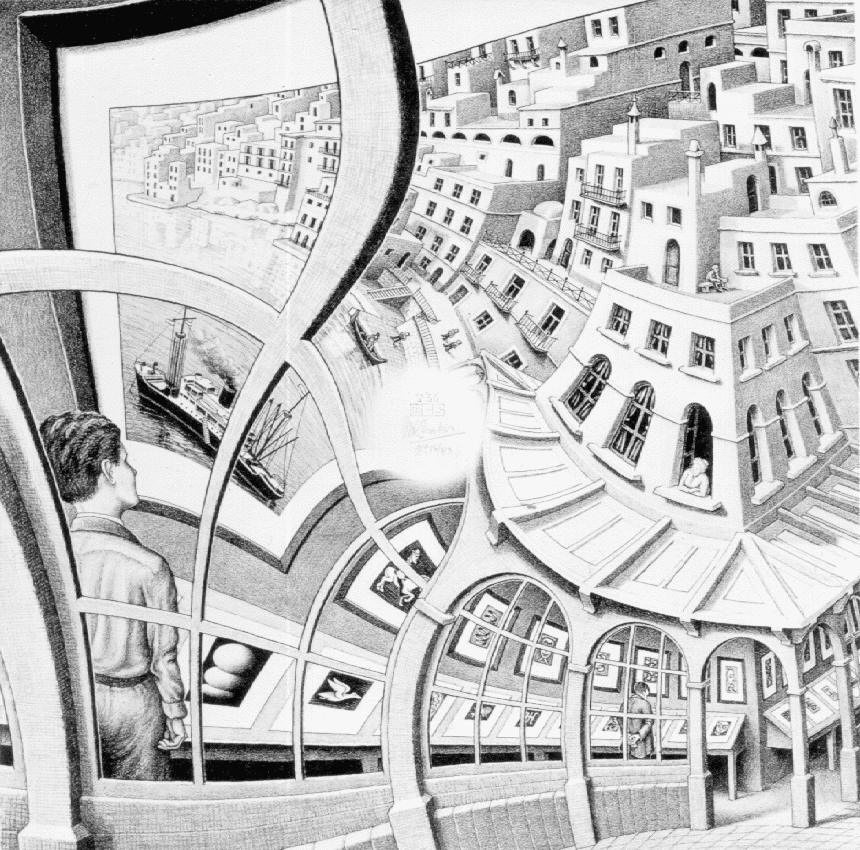
\includegraphics[width=0.5\columnwidth]{GalleriaStampe} 
% \caption[An example of a floating figure]{An example of a floating figure (a reproduction from the \emph{Gallery of prints}, M.~Escher,\index{Escher, M.~C.} from \url{http://www.mcescher.com/}).} % The text in the square bracket is the caption for the list of figures while the text in the curly brackets is the figure caption
% \label{fig:gallery} 
% \end{figure}
% 
% \lipsum[5] % Dummy text
% 
% \begin{enumerate}[noitemsep] % [noitemsep] removes whitespace between the items for a compact look
% \item First item in a list
% \item Second item in a list
% \item Third item in a list
% \end{enumerate}
% 
% %------------------------------------------------
% 
% \subsection{Paragraphs}
% 
% \lipsum[6] % Dummy text
% 
% \paragraph{Paragraph Description} \lipsum[7] % Dummy text
% 
% \paragraph{Different Paragraph Description} \lipsum[8] % Dummy text
% 
% %------------------------------------------------
% 
% \subsection{Math}
% 
% \lipsum[4] % Dummy text
% 
% \begin{equation}
% \cos^3 \theta =\frac{1}{4}\cos\theta+\frac{3}{4}\cos 3\theta
% \label{eq:refname2}
% \end{equation}
% 
% \lipsum[5] % Dummy text
% 
% \begin{definition}[Gauss] 
% To a mathematician it is obvious that
% $\int_{-\infty}^{+\infty}
% e^{-x^2}\,dx=\sqrt{\pi}$. 
% \end{definition} 
% 
% \begin{theorem}[Pythagoras]
% The square of the hypotenuse (the side opposite the right angle) is equal to the sum of the squares of the other two sides.
% \end{theorem}
% 
% \begin{proof} 
% We have that $\log(1)^2 = 2\log(1)$.
% But we also have that $\log(-1)^2=\log(1)=0$.
% Then $2\log(-1)=0$, from which the proof.
% \end{proof}
% 
% %----------------------------------------------------------------------------------------
% %	RESULTS AND DISCUSSION
% %----------------------------------------------------------------------------------------
% 
% \section{Results and Discussion}
% 
% \lipsum[10] % Dummy text
% 
% %------------------------------------------------
% 
% \subsection{Subsection}
% 
% \lipsum[11] % Dummy text
% 
% \subsubsection{Subsubsection}
% 
% \lipsum[12] % Dummy text
% 
% \begin{description}
% \item[Word] Definition
% \item[Concept] Explanation
% \item[Idea] Text
% \end{description}
% 
% \lipsum[12] % Dummy text
% 
% \begin{itemize}[noitemsep] % [noitemsep] removes whitespace between the items for a compact look
% \item First item in a list
% \item Second item in a list
% \item Third item in a list
% \end{itemize}
% 
% \subsubsection{Table}
% 
% \lipsum[13] % Dummy text
% 
% \begin{table}[hbt]
% \caption{Table of Grades}
% \centering
% \begin{tabular}{llr}
% \toprule
% \multicolumn{2}{c}{Name} \\
% \cmidrule(r){1-2}
% First name & Last Name & Grade \\
% \midrule
% John & Doe & $7.5$ \\
% Richard & Miles & $2$ \\
% \bottomrule
% \end{tabular}
% \label{tab:label}
% \end{table}
% 
% Reference to Table~\vref{tab:label}. % The \vref command specifies the location of the reference
% 
% %------------------------------------------------
% 
% \subsection{Figure Composed of Subfigures}
% 
% Reference the figure composed of multiple subfigures as Figure~\vref{fig:esempio}. Reference one of the subfigures as Figure~\vref{fig:ipsum}. % The \vref command specifies the location of the reference
% 
% \lipsum[15-18] % Dummy text
% 
% \begin{figure}[tb]
% \centering
% \subfloat[A city market.]{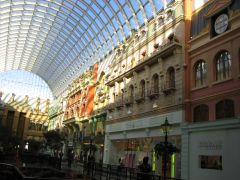
\includegraphics[width=.45\columnwidth]{Lorem}} \quad
% \subfloat[Forest landscape.]{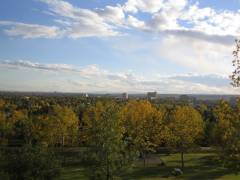
\includegraphics[width=.45\columnwidth]{Ipsum}\label{fig:ipsum}} \\
% \subfloat[Mountain landscape.]{
\includegraphics[width=.45\columnwidth]{Dolor}} \quad
% \subfloat[A tile decoration.]{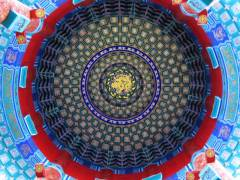
\includegraphics[width=.45\columnwidth]{Sit}}
% \caption[A number of pictures.]{A number of pictures with no common theme.} % The text in the square bracket is the caption for the list of figures while the text in the curly brackets is the figure caption
% \label{fig:esempio}
% \end{figure}
% 

%----------------------------------------------------------------------------------------
%	BIBLIOGRAPHY
%----------------------------------------------------------------------------------------
\bibliographystyle{unsrt}

\bibliography{report_biblio.bib} % The file containing the bibliography

%----------------------------------------------------------------------------------------

\end{document}
